%%
% The BIThesis Template for Bachelor Graduation Thesis
%
% 北京理工大学毕业设计（论文）第二章节 —— 使用 XeLaTeX 编译
%
% Copyright 2020-2023 BITNP
%
% This work may be distributed and/or modified under the
% conditions of the LaTeX Project Public License, either version 1.3
% of this license or (at your option) any later version.
% The latest version of this license is in
%   http://www.latex-project.org/lppl.txt
% and version 1.3 or later is part of all distributions of LaTeX
% version 2005/12/01 or later.
%
% This work has the LPPL maintenance status `maintained'.
%
% The Current Maintainer of this work is Feng Kaiyu.
\chapter{音频情绪数据集与信号处理方法}

\section{音频情绪数据集的类型与选择}

本节梳理当前语音情绪识别研究中常用的代表性公开数据集，比较与分析其基础属性。将以各数据集的语言、采集方式、情绪表达特点、用户构成、情绪标签结构、数据规模、公开访问性及可用性为中心进行比较，并在此基础上尝试归纳适合本研究的数据集选择标准。详细对比见表 \ref{tab:datasets}。

\begin{table}[!ht]
\scriptsize
\centering
\caption{语音情绪识别常用公开数据集比较} \label{tab:datasets}
\begin{tabularx}{\textwidth}{@{}l >{\raggedright\arraybackslash}p{2.2cm} l l >{\centering\arraybackslash}X >{\centering\arraybackslash}X c@{}}
\toprule
\textbf{类别} & \textbf{数据集} & \textbf{语言} & \textbf{规模} & \textbf{标签构成} & \textbf{对话上下文} & \textbf{多模态} \\ \midrule
表演型 & RAVDESS & 英语 & 7,356条 & 离散类(8) & 低 & 是 \\ \midrule
表演型 & EMO-DB & 德语 & 约535条 & 离散类(7) & 低 & 否 \\ \midrule
表演型 & SAVEE & 英语 & 480条 & 离散类(7) & 低 & 是 \\ \midrule
表演型 & TESS & 英语 & 2,800条 & 离散类(7) & 低 & 否 \\ \midrule
表演型 & CREMA-D & 英语 & 7,442条 & 离散类(6) & 低 & 是 \\ \midrule
表演型 & CASIA & 汉语 & 约1,200条 & 离散类(6) & 低 & 否 \\ \midrule
对话型 & IEMOCAP & 英语 & 约12小时 & 离散+连续类 & 高 & 是 \\ \midrule
诱导型 & MSP-IMPROV & 英语 & 约9小时 & 离散类 & 高 & 是 \\ \midrule
自然型 & MSP-Podcast & 英语 & 409小时 & 离散+连续类 & 中-高 & 否 \\ \midrule
对话型 & MELD & 英语 & 1.3万条 & 离散类 & 高 & 是 \\ \midrule
自然型 & FAU Aibo & 德语 & 约9小时 & 离散类 & 中等 & 否 \\ \midrule
交互型 & RECOLA & 法语 & 多模态 & 连续类 & 高 & 是 \\ \midrule
诱导型 & eNTERFACE & 英语 & 音视频 & 离散类 & 低 & 是 \\ \midrule
半自然 & ShEMO & 波斯语 & 3,000条 & 离散类 & 低 & 否 \\ \midrule
现实自然 & EMOVOME & 西班牙语 & 999条 & 离散+连续类 & 中等 & 否 \\ \midrule
自然型 & CNSCED & 汉语 & 14小时 & 多维度离散类(6) & 中等 & 否 \\ \bottomrule
\end{tabularx}
\end{table}

从表 \ref{tab:datasets} 可见，语音情绪数据集在采集方式、标签形式、语言环境和用户构成上存在差异。表演型数据集通常在受控环境下采集，情绪标签较为明确，便于开展基础分类实验。对话型和自然型数据集更接近实际应用场景，但情绪边界、上下文因素和标注一致性也更加复杂。离散情绪标签适合多分类任务，连续维度标签则更适合回归或维度情绪建模。数据集差异不仅体现在规模上，也影响任务定义、评价方式和结果可比性\cite{ma2023review,pappagari2023music}。

本研究在数据集选择时主要考虑公开访问性、标签清晰度、用户构成、数据规模和基准可比性。数据集需要能够稳定获取，并支持后续实验复现。标签体系应适合语音情绪分类。用户数量和性别分布不宜过度偏斜。数据规模应能支撑基础实验，同时避免预处理和模型验证过于复杂。

基于上述标准，本研究首先选择RAVDESS作为基础实验数据集。RAVDESS可公开访问，性别分布较为均衡，情绪类别构成清晰，在语音情绪识别研究中也较为常用，便于后续实验结果分析与比较。该数据集属于受控环境下的表演型基准数据集，与自然场景语音仍存在差异。本文将其作为主要实验基础，其适用范围主要对应受控语音条件下的模型比较。


\section{信号处理技术}

\subsection{信号预处理}

\textbf{(1) 输入格式统一：重采样与通道统一}

不同语音数据集的音频文件可能具有不同的采样频率（如16 kHz、44.1 kHz等）和通道配置（单声道/立体声），这些差异会影响可分析的频率范围与后续特征分布。重采样（resampling）将信号从原始采样频率转换至目标采样频率，下采样时需先通过低通滤波器抑制高频成分以避免混叠。对于立体声输入，通常取左右声道平均值转换为单声道：
\begin{equation}
x_{\text{mono}}[n] = \frac{x_L[n] + x_R[n]}{2}
\end{equation}
其中 $x_L[n]$ 和 $x_R[n]$ 分别为左右声道信号。统一采样频率与通道格式有助于保证后续特征提取输入条件的一致性，避免模型将设备差异作为情绪信息学习\cite{leem2024selective,lin2023chunk}。

\textbf{(2) 振幅归一化}

不同语音文件因用户发声音量、麦克风灵敏度、设备增益等差异，振幅范围可能不一致。振幅归一化（amplitude normalization）用于统一输入信号的振幅范围，减少录音条件差异对特征分布的影响\cite{fan2022isnet,lin2023chunk}。常用方法包括峰值归一化与均方根归一化（RMS normalization）。峰值归一化以信号最大绝对值为基准缩放，计算简单但对瞬时峰值敏感；RMS 归一化以信号平均强度为基准：
\begin{equation}
x_{\text{rms}}[n] = \frac{x[n]}{\sqrt{\frac{1}{N}\sum_{n=0}^{N-1} x[n]^2} + \varepsilon}
\end{equation}
其中 $\varepsilon$ 为防止分母为零的极小常数，通常可提供较为稳定的幅度调节效果\cite{zhang2020transfer,leem2024selective,lin2023chunk}。需要注意的是，情绪表达本身包含发声强度线索（如愤怒伴随较高强度、悲伤呈现较低强度），应用归一化时需在减少录音条件差异与保留情绪相关强度信息之间取得平衡\cite{fan2022isnet,zhang2020transfer}。



\subsection{时频变换与频谱分析}

\textbf{(1) 分帧与帧重叠：时间分辨率与频率分辨率的权衡}

设离散语音信号长度为 $N$，记作 $x[n]$，帧长为 $L$，帧移（hop size）为 $H$，则第 $m$ 帧可表示为：
\begin{equation}
x_m[n] = x[mH+n], \qquad 0 \le n < L
\end{equation}
其中 $x[n]$ 为原始离散语音信号，$x_m[n]$ 为第 $m$ 帧，$L$ 为帧长（样本数），$H$ 为帧移，$m$ 为帧索引。总帧数 $M$ 通常按下式计算：
\begin{equation}
M = \left\lfloor \frac{N-L}{H} \right\rfloor + 1
\end{equation}
其中 $\lfloor\cdot\rfloor$ 为向下取整函数。上述公式表示从长度为 $N$ 的信号中以帧移 $H$ 滑动提取长度为 $L$ 的帧所能得到的帧数。

例如，当采样频率 $F_s = 16\,\text{kHz}$ 时，25 ms 帧对应约 400 个样本，10 ms 帧移对应约 160 个样本。帧重叠是指相邻帧之间存在公共区间，即 $H < L$ 的情形。重叠率可表示为：
\begin{equation}
r = 1 - \frac{H}{L}
\end{equation}
例如 $L=400$、$H=160$ 时，重叠率为 60\%。采用帧重叠的目的是避免相邻帧之间信息断裂，使时间轴上的变化更为平滑稳定。重叠率过小可能导致帧间连续性不足，过大则会增加计算量并引入过多冗余信息。

帧长与帧移共同决定了时间分辨率与频率分辨率之间的权衡。通常，帧移越小，时间轴上的分析越密集，时间分辨率越高，上述关系可近似表示为：
\begin{equation}
\Delta t \approx \frac{H}{F_s}
\end{equation}
其中 $\Delta t$ 为相邻分析点的时间间隔。频率分辨率则与快速傅里叶变换（Fast Fourier Transform, FFT）长度相关：
\begin{equation}
\Delta f \approx \frac{F_s}{N_{\mathrm{FFT}}}
\end{equation}
其中 $\Delta f$ 为频率 bin 间隔，$N_{\mathrm{FFT}}$ 为快速傅里叶变换长度。帧长过短虽能提升时间分辨率，但会降低频率分辨率，难以刻画精细的频谱结构；帧长过长虽能提高频率分辨率，但可能破坏帧内信号的准平稳性。

从语音情绪识别的视角来看，分帧与重叠涉及计算层面的处理，也直接关系到情绪信息的保留。情绪表达通常并非均匀分布于整段语音，而往往集中于特定的时间区间（如抑扬变化、能量突增、停顿等）\cite{mirsamadi2017automatic,lin2023chunk,peng2021efficient}。合理设定帧参数有助于保留这些时间相关的情绪线索，并为后续的时频变换提供稳定的基础。

\textbf{(2) 傅里叶变换：从时域到频域的基础}

分析语音信号的频率结构，常用的方法之一是傅里叶变换。时域波形包含发声强度、周期性、共振特性、频带能量分布等信息，但仅从时域难以直观解读这些内容。在语音情绪识别中，基频、共振峰、频谱斜率、频带能量分布等频域线索具有一定作用。将时域信号转换为频域表示，是需要关注的基础步骤之一。傅里叶变换为后续的短时傅里叶变换、谱图以及梅尔系列特征提取提供了理论基础。

对于长度为 $N$ 的离散信号 $x[n]$，其离散傅里叶变换（Discrete Fourier Transform, DFT）定义为：
\begin{equation}
X[k] = \sum_{n=0}^{N-1} x[n] e^{-j 2\pi kn/N}, \qquad 0 \le k < N
\end{equation}
其中 $x[n]$ 为时域离散信号，$X[k]$ 为第 $k$ 个频率 bin 的复数谱值，$N$ 为变换长度，$j$ 为虚数单位，$k$ 为频率 bin 索引。

复数谱包含幅度与相位信息。幅度谱可由下式计算：
\begin{equation}
|X[k]| = \sqrt{\Re(X[k])^2 + \Im(X[k])^2}
\end{equation}
其中 $\Re(X[k])$、$\Im(X[k])$ 分别为 $X[k]$ 的实部与虚部。

功率谱通常定义为：
\begin{equation}
P[k] = |X[k]|^2
\end{equation}

频率 bin $k$ 对应的实际频率近似为：
\begin{equation}
f_k = \frac{k F_s}{N}
\end{equation}
其中 $F_s$ 为采样频率。上述公式表明离散傅里叶变换将时域信号分解为频率轴上的离散分量。

在语音情绪识别中，离散傅里叶变换与快速傅里叶变换是获取频域信息的基础方法之一。但离散傅里叶变换对整个信号进行一次变换，难以直接反映频率结构随时间的变化。例如，同一段语音中，起始与结尾的基频、能量分布可能不同，而单次离散傅里叶变换会将这些差异平均化。与对整段语音进行一次傅里叶变换相比，采用短时傅里叶变换进行逐帧分析相对更为重要。傅里叶变换是解析语音频率结构的基本工具，快速傅里叶变换则是其实用化计算的关键算法。

\begin{figure}[htbp]
    \centering
    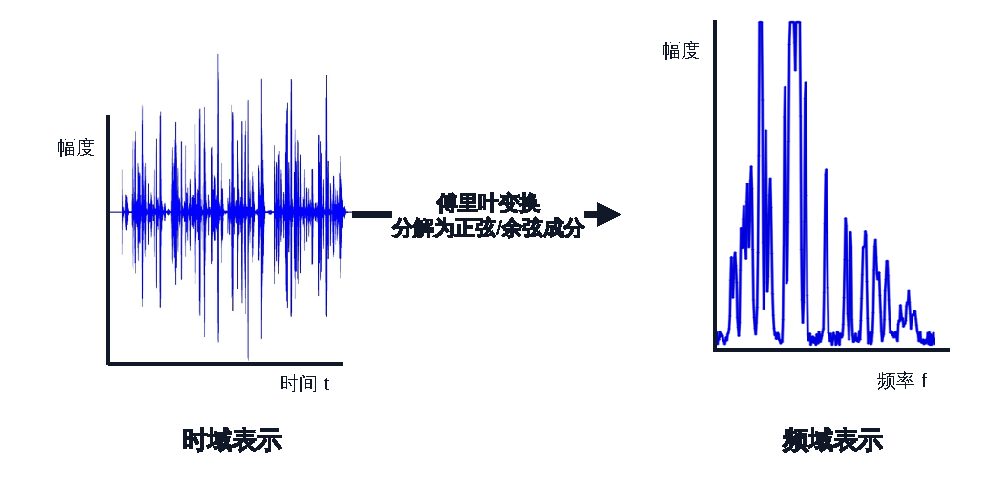
\includegraphics[width=0.75\textwidth]{images/feedback_diagrams/chapter2/fourier/ft_time_to_frequency.drawio.pdf}
    \caption{傅里叶变换将时域波形转换为频域幅度谱的直观过程}
    \label{fig:ft_time_to_frequency}
\end{figure}

图\ref{fig:ft_time_to_frequency}以一段语音波形为例，展示傅里叶变换如何把时间轴上的振幅变化转换为频率轴上的幅度分布。该图对应前文离散傅里叶变换公式中的时域输入与频域分量，有助于理解后续短时分析为何需要保留时间位置。

\textbf{(3) 窗函数：频谱泄漏抑制与频率分辨率权衡}

在处理语音数据的时候，傅里叶变换可以将语音信号从时间幅度函数变换为时间频率的函数，但是傅里叶变换会在帧的起始与结束位置产生不连续性。这种不连续性是由于实际信号被截断为有限长度所致。这种边界不连续会导致频谱泄漏，使得频谱展宽并引起相邻频率成分的相互干扰。为减轻这一影响，需要对每一帧乘以窗函数，这一过程称为加窗。

将窗函数 $w[n]$ 作用于第 $m$ 帧 $x_m[n]$，得到加窗后的信号：
\begin{equation}
x_m^{(w)}[n] = x_m[n] \cdot w[n], \qquad 0 \le n < L
\end{equation}
其中 $x_m[n]$ 为原第 $m$ 帧，$w[n]$ 为长度为 $L$ 的窗函数，$x_m^{(w)}[n]$ 为加窗后的帧。

在时域乘以窗函数等价于在频域进行卷积，即：
\begin{equation}
X_m^{(w)}(\omega) = X_m(\omega) * W(\omega)
\end{equation}
其中 $X_m(\omega)$ 为原帧的频谱，$W(\omega)$ 为窗函数的频谱，$*$ 为卷积运算。窗函数的形状决定了其主瓣宽度与旁瓣衰减特性，从而影响泄漏抑制程度与频率分辨率。


汉明窗定义为：
\begin{equation}
w_{\mathrm{Ham}}[n] = 0.54 - 0.46\cos\left(\frac{2\pi n}{L-1}\right), \qquad 0 \le n < L
\end{equation}
汉宁窗定义为：
\begin{equation}
w_{\mathrm{Hann}}[n] = 0.5\left(1-\cos\left(\frac{2\pi n}{L-1}\right)\right), \qquad 0 \le n < L
\end{equation}
其中 $L$ 为窗长，$n$ 为窗内样本索引。这两类窗函数能平滑帧两端，有效抑制频谱泄漏，较矩形窗在频谱泄漏抑制方面更为有效。汉明窗在泄漏抑制与频率分辨率之间取得较好平衡，在语音特征提取中较为常见。汉宁窗同样具有平滑特性，且窗端衰减更平缓。

对于语音情绪识别，整体声学模式的稳定性通常比精确跟踪单一频谱峰值更受关注，汉明窗在相关任务中较为常见。



\textbf{(4) 短时傅里叶变换：时频分析的桥梁}

离散傅里叶变换能够揭示信号的频率构成，但难以直接反映频率结构随时间的变化。语音信号具有时变特性，情绪表达体现在特定时间区间的语调变化、能量转移、共振结构演变等方面。在语音情绪识别中，频率信息需要和时间变化趋势共同分析。短时傅里叶变换为此目的而引入，通过对短时区间逐段进行傅里叶变换，同时呈现信号的时间与频率分布。

短时傅里叶变换可理解为对信号施加滑动窗，并对每个窗内分段进行傅里叶变换。该变换的一般形式可表示为：
\begin{equation}
X(m,k) = \sum_{n=-\infty}^{\infty} x[n] \cdot w[n-mH] \cdot e^{-j 2\pi kn/N}
\end{equation}
其中 $x[n]$ 为原始离散信号，$w[n-mH]$ 为移动至第 $m$ 个时间位置的窗函数，$H$ 为帧移，$N$ 为快速傅里叶变换长度，$m$ 为时间帧索引，$k$ 为频率 bin 索引。

结合前述分帧处理，短时傅里叶变换可视为”分帧—加窗—逐帧快速傅里叶变换”的连续过程。

短时傅里叶变换能够同时提供时间与频率信息，但该变换的时间分辨率与频率分辨率之间往往存在权衡。采用较短的窗函数可获得较好的时间分辨率，但频率分辨率可能相应降低；采用较长的窗函数则可获得更精细的频率结构，但对时间变化的响应能力相对较弱。上述时间分辨率与频率分辨率之间的权衡关系与帧移、快速傅里叶变换长度及采样频率等因素密切相关。

在语音情绪识别中，短时傅里叶变换可同时保留随时间演变的声学模式。例如，愤怒或喜悦可能伴随特定区间的能量聚集与快速的语调变化，而悲伤则可能表现为相对平缓的频谱演变。短时傅里叶变换可同时保留这些时变模式，从而为后续的谱图、对数梅尔谱（log-Mel spectrogram）及梅尔频率倒谱系数等特征提取提供基础。短时傅里叶变换是连接语音时域与频域分析的重要中间表示之一，能够在一定程度上反映情绪表达中的时变特性。

\begin{figure}[htbp]
    \centering
    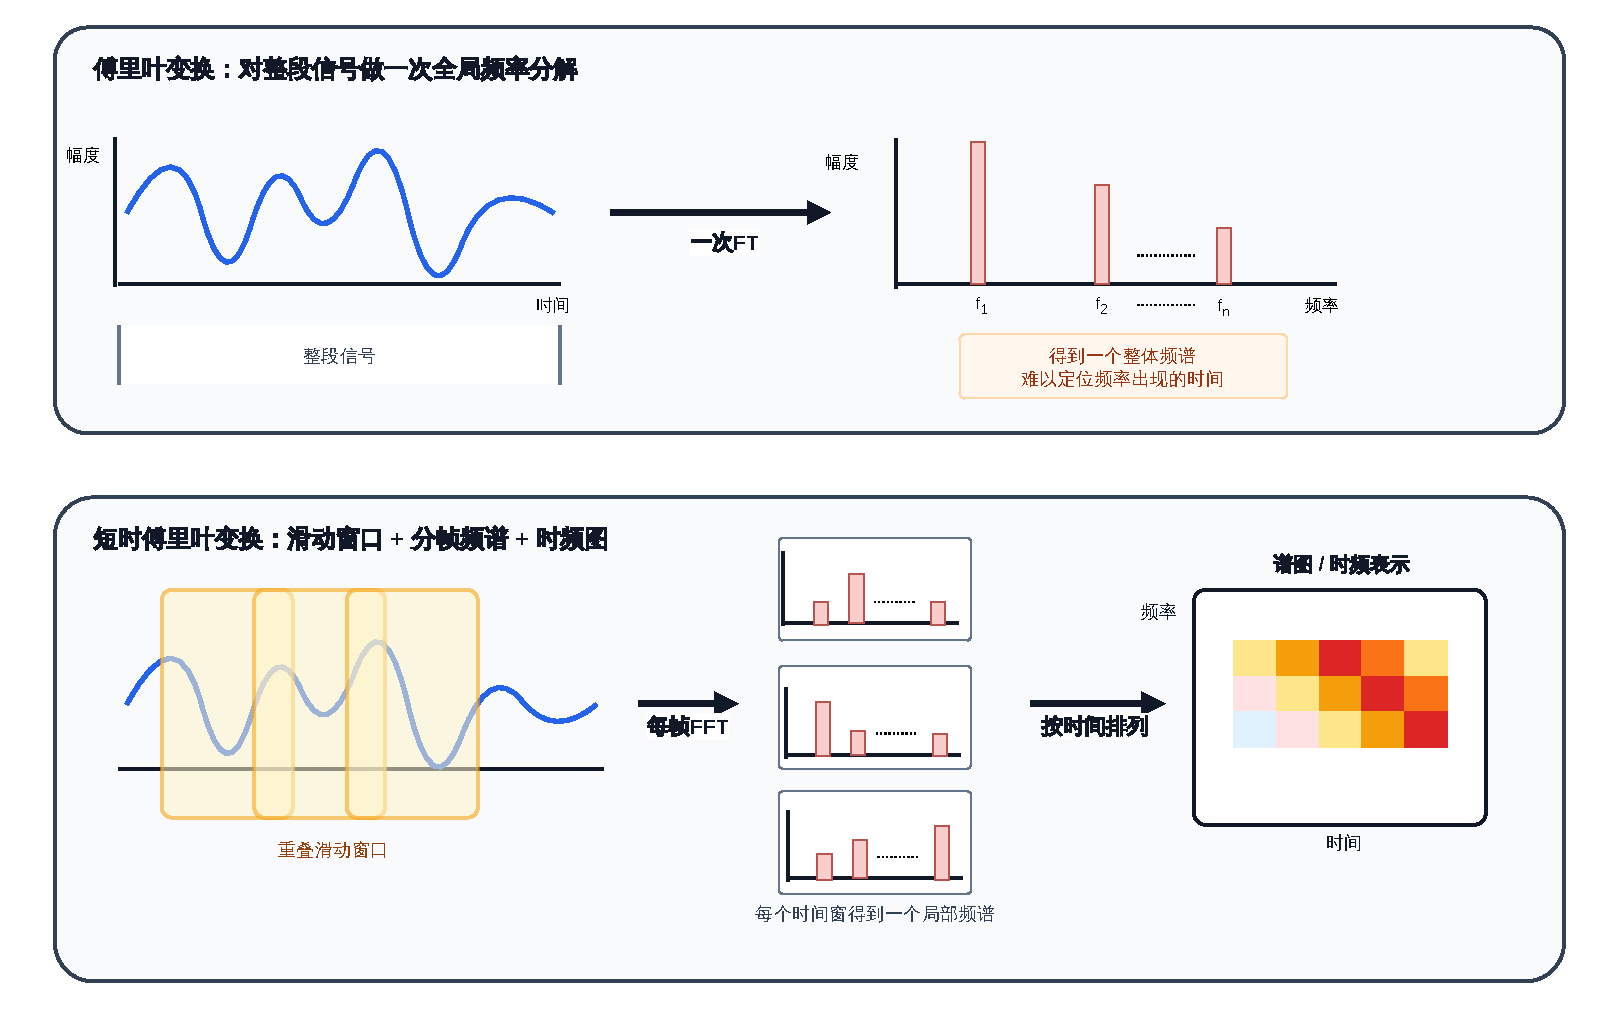
\includegraphics[width=0.75\textwidth]{images/feedback_diagrams/chapter2/stft/ft_vs_stft.drawio.pdf}
    \caption{傅里叶变换与短时傅里叶变换在时间信息保留方式上的差异}
    \label{fig:ft_vs_stft}
\end{figure}

图\ref{fig:ft_vs_stft}对比了整段傅里叶变换与短时傅里叶变换的差异。前者得到全局频谱。后者通过滑动窗口形成按时间排列的局部频谱，更适合描述语音情绪线索随时间变化的情况。


\textbf{(5) 频谱图：时频表示的三种形式}

短时傅里叶变换的输出为复数矩阵，该矩阵的维度分别为时间索引 $m$ 与频率索引 $k$。该复数表达在数学上是完整的，但在实际语音分析或模型输入中，通常将其转换为幅度或能量形式。谱图（spectrogram）即为此类时间-频率表示，同时呈现时间轴、频率轴以及各时频位置的强度，可较为清晰地展示语音信号的结构变化。

一种基本形式是幅度谱图，使用短时傅里叶变换结果的绝对值：
\begin{equation}
S_{\mathrm{mag}}(m,k) = |X(m,k)|
\end{equation}
其中 $X(m,k)$ 为短时傅里叶变换结果，$S_{\mathrm{mag}}(m,k)$ 为幅度谱图值。幅度谱图反映各时频位置的振幅大小，可较为清晰地观察不同频带的相对强度差异。

功率谱图（power spectrogram）则使用幅度的平方，从能量角度进行表示：
\begin{equation}
S_{\mathrm{pow}}(m,k) = |X(m,k)|^2
\end{equation}
功率谱图与信号的能量分布较为密切地相关，在许多声学特征提取中作为基础输入使用。在语音处理中，功率形式往往比幅度形式较为常见，后续的梅尔滤波器组（Mel filterbank）运算也通常基于功率谱图进行。

对数谱图（log spectrogram）通过对功率谱图取对数，压缩动态范围，使其更接近人耳听觉感知特性：
\begin{equation}
S_{\log}(m,k) = \log\left(S_{\mathrm{pow}}(m,k)+\varepsilon\right)
\end{equation}
其中 $\varepsilon$ 为极小常数，用于避免数值不稳定。实际实现中也常采用 dB 刻度 $10\log_{10}(\cdot)$，对数刻度能够压缩大动态范围，使微弱频率成分相对更易被观测。

谱图是语音情绪识别中较为常用的输入表示之一\cite{peng2021efficient,mirsamadi2017automatic,chen2023dwformer}。不同情绪状态下，特定频带的能量分布、谱包络、共振结构及发声强度的时变模式可能有所不同，谱图能够较为清晰地呈现这些差异。在卷积神经网络类模型中，常将谱图视作二维图像，自动学习具有情绪判别性的时频模式\cite{zhang2023cnn,wang2024swin}。此外，对数谱图是后续梅尔滤波器组、对数梅尔谱及梅尔频率倒谱系数等特征构建的基础。

谱图本身并不总是适合直接作为最终输入。线性频率轴难以直接反映人耳的非线性感知特性，高频区域分布了较多频率 bin\cite{chen2023dwformer}。同时，谱图的分辨率与分布受短时傅里叶变换参数、窗长、帧移及变换长度等因素影响\cite{peng2021efficient}。谱图是重要的中间表示，在实际应用中还可进一步转换为梅尔尺度或倒谱系数等更具感知适应性的特征\cite{pappagari2023music}。

\begin{figure}[htbp]
    \centering
    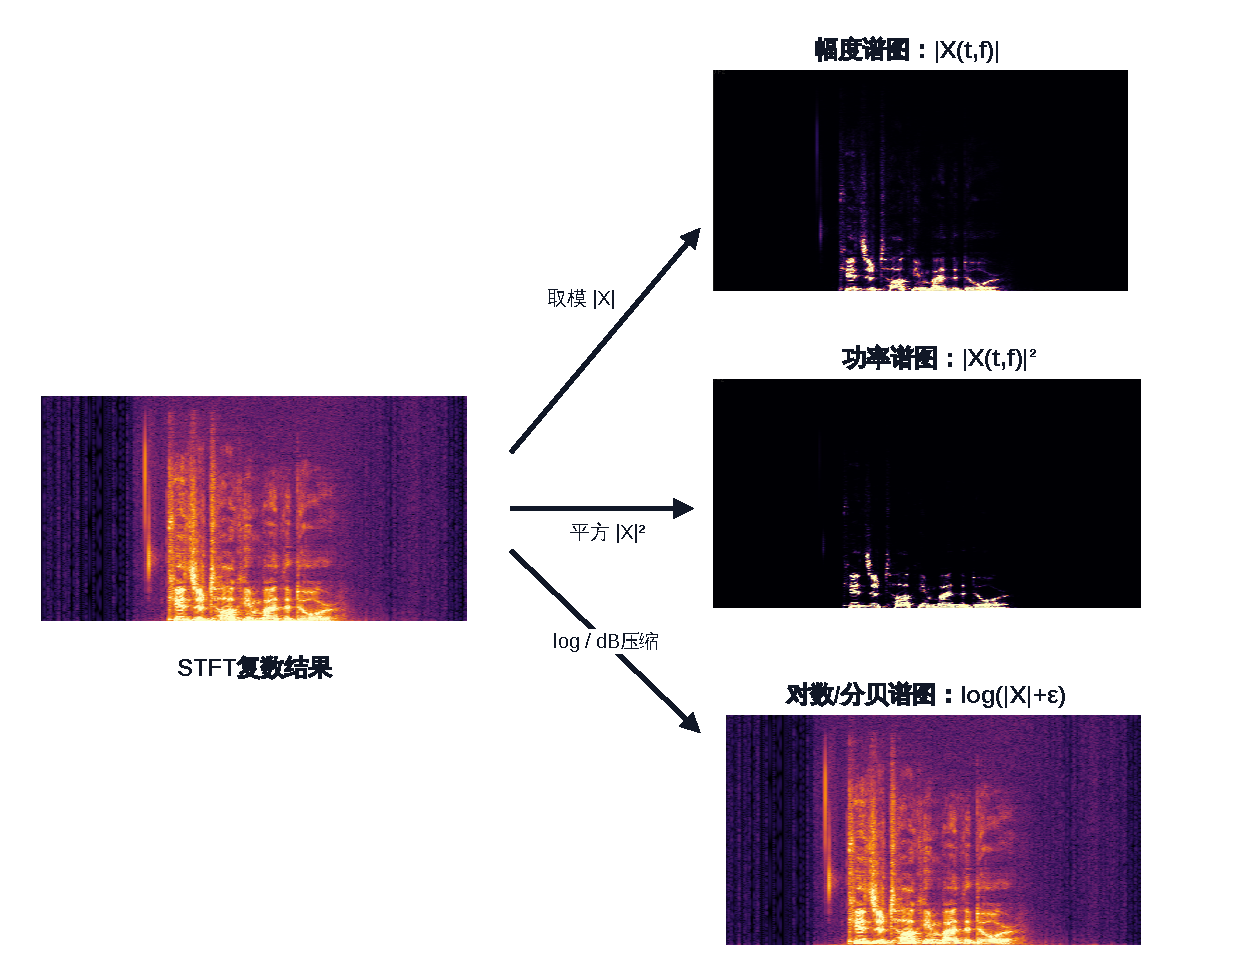
\includegraphics[width=0.75\textwidth]{images/feedback_diagrams/chapter2/spectrogram_forms/spectrogram_forms.drawio.pdf}
    \caption{幅度谱图、功率谱图与对数谱图在同一时频结构上的显示差异}
    \label{fig:spectrogram_forms}
\end{figure}

图\ref{fig:spectrogram_forms}在同一时频结构上展示幅度谱图、功率谱图和对数谱图的显示差异。三类表示的时间轴与频率轴保持一致，区别主要体现在每个时频位置强度值的计算方式与动态范围压缩程度。


\subsection{感知特征提取}

\textbf{(1) Mel尺度与梅尔滤波器组}

为弥补线性频率轴无法直接反映人耳听觉特性的不足，常采用梅尔尺度（Mel scale）。这是一种模拟人耳听觉感知的非线性频率刻度。线性频率 $f$（单位 Hz）与梅尔频率 $m$ 之间的典型转换关系为：
\begin{equation}
m = 2595 \log_{10}\left(1+\frac{f}{700}\right)
\end{equation}

该转换在低频区域保持相对较高的分辨率，在高频区域逐渐压缩，从而构建出更贴近听觉感知的频率轴。在语音情绪识别中，梅尔尺度有助于以类人耳的方式重构语调、共振、频带能量分布等情绪相关线索\cite{pappagari2023music,peng2021efficient}。

梅尔滤波器组是将梅尔尺度应用于特征提取的具体方法。通常在线性频率轴上按梅尔间隔布置多个三角形滤波器，每个滤波器对相应频带的能量进行汇总。设第 $p$ 个梅尔滤波器为 $H_p[k]$，则第 $m$ 帧第 $p$ 个梅尔频带的能量为：
\begin{equation}
E_p(m) = \sum_{k=0}^{N-1} |X(m,k)|^2 H_p[k]
\end{equation}
其中 $|X(m,k)|^2$ 为第 $m$ 帧第 $k$ 个频率 bin 的功率谱值，$N$ 为频率 bin 总数。

梅尔滤波器组的作用在于将相邻频率区间按听觉感知特性进行整合，从而将原始精细的线性频谱压缩为相对稳定、具有感知意义的频带能量表示\cite{peng2021efficient,chen2023dwformer}。该过程具有多个优点：一是提供更贴近人耳感知的频域表达；二是通过频带能量聚合，能在一定程度上降低噪声敏感性；三是作为对数梅尔谱和梅尔频率倒谱系数等特征的基础，可较为便捷地与后续处理结合。

梅尔滤波器组会丢失部分精细的频率结构，对于需要精确分析窄带成分的任务可能存在局限。在语音情绪识别中，整体能量分布与听觉相似性往往更受关注，梅尔特征仍较为常见\cite{hao2024channel,pappagari2023music,peng2021efficient}。


\textbf{(2) 对数梅尔谱图：听觉感知与时频表示的融合}

对梅尔滤波器组输出的各帧频带能量取对数，即得到对数梅尔谱图。可理解为将基于短时傅里叶变换的功率谱映射至梅尔刻度后，再通过对数运算压缩动态范围。对数梅尔谱图既模拟了人耳的非线性听觉特性，又通过对数变换使能量分布更为平稳。

以前述梅尔滤波器组输出能量 $E_p(m)$ 为基础，对其取对数得到第 $m$ 帧第 $p$ 个梅尔频带的对数能量：
\begin{equation}
M_p(m) = \log\left(E_p(m)+\varepsilon\right)
\end{equation}
其中 $M_p(m)$ 为对数梅尔谱值，$\varepsilon$ 为极小常数。实际应用中也可采用 dB 刻度 $10\log_{10}(\cdot)$。

语音信号的能量动态范围较广。原始功率谱或梅尔滤波器组输出中，某些频带能量可能远大于其他频带，若未经处理直接使用，模型可能过度关注大值区域。对数变换可压缩动态范围，使小能量差异也能被有效保留，同时与人耳的对数响度感知特性有一定关联。对数梅尔谱是数值处理结果，也是连接物理信号与听觉感知的常用表示之一\cite{he2023multiple,peng2021efficient,wang2024swin}。

例如，愤怒或喜悦常伴随能量聚集与快速语调变化，而悲伤则可能表现为相对平缓的频谱演变。对数梅尔谱图能够以较为清晰的二维形式呈现这些差异，适合卷积神经网络或注意力机制学习局部模式与关键区域\cite{peng2021efficient,zhang2023cnn,wang2024swin}。尽管近年来也出现未经处理直接使用原始波形的端到端方法，但对数梅尔谱图仍是目前较为稳定、较为常用的基线特征之一\cite{pappagari2023music}。

\begin{figure}[htbp]
    \centering
    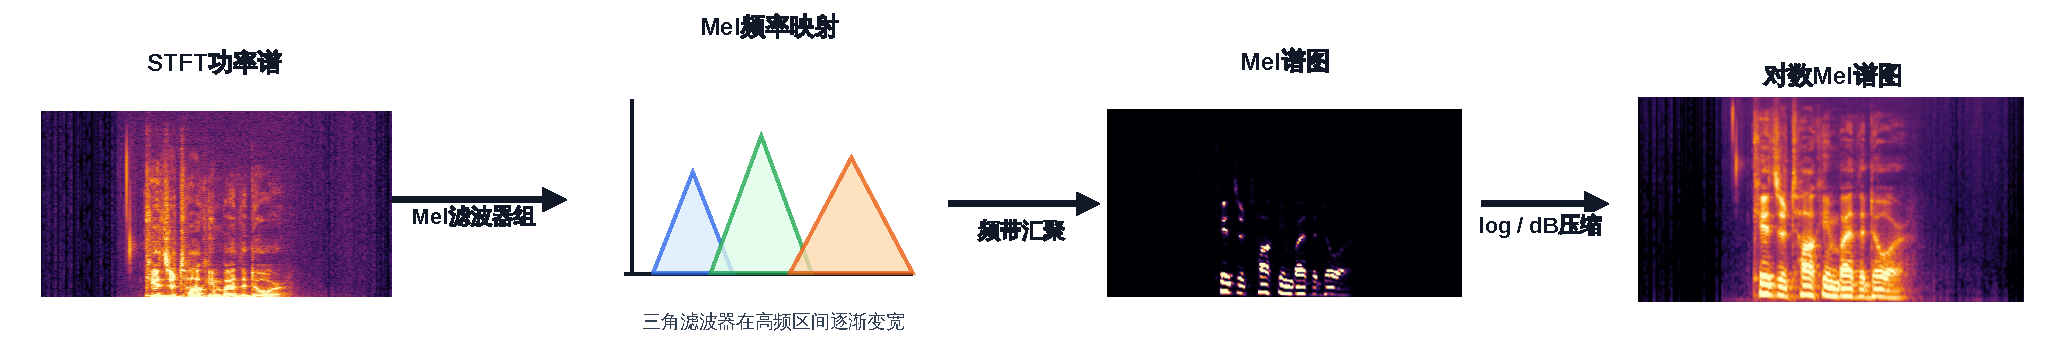
\includegraphics[width=0.75\textwidth]{images/feedback_diagrams/chapter2/logmel/mel_vs_logmel.drawio.pdf}
    \caption{梅尔谱图与对数梅尔谱图的生成关系及动态范围差异}
    \label{fig:mel_vs_logmel}
\end{figure}

图\ref{fig:mel_vs_logmel}展示从短时功率谱到梅尔谱图，再到对数梅尔谱图的生成关系。梅尔滤波器组用于把线性频率轴上的能量汇聚到听觉频带。对数压缩则用于减小能量动态范围。

\begin{figure}[htbp]
    \centering
    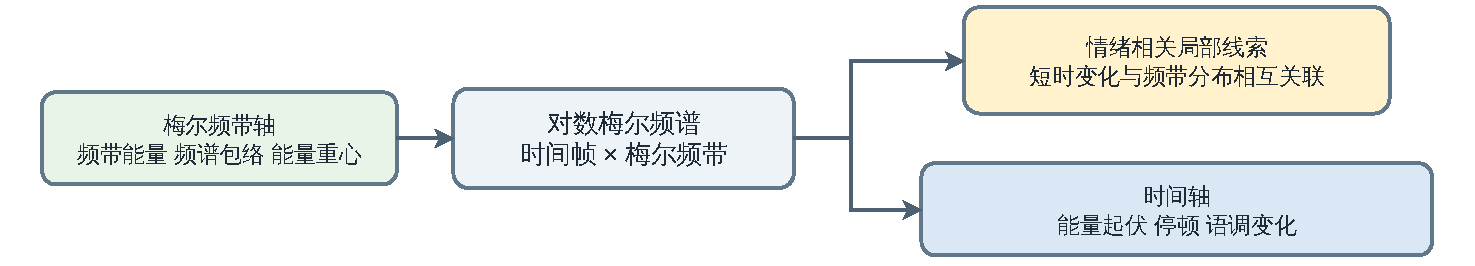
\includegraphics[width=0.75\textwidth]{images/chapter2/chapter2_logmel_time_frequency.drawio.pdf}
    \caption{对数梅尔频谱的时间-频带结构与情绪线索表达}
    \label{fig:chapter2_logmel_time_frequency}
\end{figure}

图\ref{fig:chapter2_logmel_time_frequency}进一步把对数梅尔频谱解释为由时间帧和梅尔频带构成的二维表示。时间轴主要保留能量起伏、停顿和语调变化，频带轴主要保留频带能量、频谱包络和能量重心。这些信息共同构成后续模型学习的声学输入基础。

对数梅尔谱图也存在一定的局限。梅尔刻度的信息压缩会损失部分线性频率轴的细节，滤波器数量、快速傅里叶变换长度、帧移、窗长等参数的选择也会影响最终特征的分辨率与分布\cite{peng2021efficient,chen2023dwformer}。实际应用中需根据具体数据集与模型结构设置参数。


\textbf{(3) 梅尔频率倒谱系数：从谱包络到紧凑特征}

前文所述的对数梅尔谱图能反映人耳听觉特性，但仍保留了各梅尔频带的能量值。在传统语音处理中，将整体谱包络压缩为低维表示往往比直接使用频带能量更便于建模。梅尔频率倒谱系数是较为常用的倒谱特征，通过对梅尔滤波器组输出的对数能量进行离散余弦变换（Discrete Cosine Transform, DCT）得到。梅尔频率倒谱系数可视为将对数梅尔谱进一步压缩为紧凑系数向量的结果。

设第 $m$ 帧第 $p$ 个梅尔频带的对数能量为 $M_p(m)$，则第 $q$ 个梅尔频率倒谱系数通常计算如下：
\begin{equation}
c_q(m) = \sum_{p=1}^{P} M_p(m) \cos\left[\frac{\pi q}{P}\left(p-\frac{1}{2}\right)\right], \qquad 0 \le q < Q
\end{equation}
其中 $c_q(m)$ 为第 $m$ 帧第 $q$ 个梅尔频率倒谱系数，$P$ 为梅尔滤波器总数，$Q$ 为保留的系数个数。

在语音处理实践中，常保留前若干阶系数。低阶系数主要反映谱包络的整体形状，而高阶系数对细节变化和噪声相对更为敏感\cite{ma2023review,pappagari2023music,peng2021efficient}。

在语音情绪识别中，梅尔频率倒谱系数是较为常用的特征之一：不同情绪状态下的共振结构、谱斜率、能量分布等特征可能不同，该特征可将这些变化归纳为相对稳定的低维表示，从而在小规模数据条件下也能提供较为可靠的基线。近年来，梅尔频率倒谱系数仍较为常见地用于基准对比或作为卷积神经网络的二维输入之一\cite{ma2023review,pappagari2023music,peng2021efficient}。

梅尔频率倒谱系数也存在局限。作为一种谱包络的压缩表示，该特征往往难以保留对数梅尔谱图中保留的部分精细时频结构。此外，该特征的最终表现受滤波器个数、系数阶数、帧长、帧移等参数影响，高阶系数的取舍需根据具体任务合理设置。梅尔频率倒谱系数在一定条件下可作为有效特征，但其适用性取决于数据规模、模型结构及任务特点\cite{peng2021efficient,chen2023dwformer}。



\subsection{特征后处理与序列长度处理}

\textbf{(1) 特征归一化：方法、统计量范围与权衡}

在语音情绪识别中，特征归一化被视为缩小不同维度特征之间尺度差异、提高学习过程中数值稳定性与收敛性的重要步骤\cite{ma2023review,leem2024selective,lin2023chunk}。不同类别的语音特征在数值范围与分布上可能存在较大差异。例如，对数梅尔能量、梅尔频率倒谱系数、基频、能量、时长等特征的量纲与分布特性各不相同\cite{pappagari2023music,peng2021efficient}。若未经归一化处理，某些维度的数值差异可能对模型训练产生较大影响\cite{zhang2020transfer}。归一化可视为在数值调整的基础上，将不同特征维度重新映射至可比且可学习范围的过程。

本文使用的Z-score 归一化（Z-score normalization）是语音情绪识别中较为常用的归一化方法之一\cite{zhang2020transfer,leem2024selective}。该方法将各特征值线性变换为均值为 0、标准差为 1 的分布，定义如下：

\begin{equation}
z = \frac{x-\mu}{\sigma + \varepsilon}
\end{equation}

其中 $x$ 为原始特征值，$\mu$ 为均值，$\sigma$ 为标准差，$z$ 为归一化后的值，$\varepsilon$ 为防止分母为零的极小常数。

该变换将输入特征进行中心化与尺度统一。在使用基于梯度的学习模型时，若输入分布存在一定偏斜或各维度尺度差异较大，训练过程可能出现不稳定的情况。在此类场景下，Z-score 归一化被视为语音处理中较为常用的预处理方式之一\cite{zhang2020transfer,leem2024selective,lin2023chunk}。

\textbf{(2) 输入长度处理：填充、截断 与 分段}

在语音情绪识别中，语音信号的时长并非固定不变，不同样本的发话长度存在一定的差异。大多数深度学习模型采用 mini-batch 方式进行训练，要求同一批次内的输入维度保持一致\cite{zhang2020transfer,leem2024selective}。如何将可变长度的序列转换为固定格式，是需要关注的问题。填充、截断 与 分段 是处理该问题的三种常用方法\cite{ma2023review,lin2023chunk,peng2021efficient}。这三种方法均旨在调整输入长度，但在信息保留方式及对模型输入结构的影响上存在差异。

填充 是较为常用的方法之一，即在较短的序列末尾或特定位置填充零值或常数，使其达到目标长度\cite{ma2023review,lin2023chunk,peng2021efficient}。设长度为 $T$ 的特征序列 $\mathbf{x}_t \in \mathbb{R}^d$ 需填充至目标长度 $T_{\max}$，则填充后的序列 $\tilde{\mathbf{x}}_t$ 可定义如下：

\begin{equation}
\tilde{\mathbf{x}}_t =
\begin{cases}
\mathbf{x}_t, & 0 \le t < T \\
\mathbf{0}, & T \le t < T_{\max}
\end{cases}
\end{equation}


其中 $\mathbf{x}_t$ 为原始时刻 $t$ 的特征向量，$\tilde{\mathbf{x}}_t$ 为填充后的特征向量，$d$ 为特征维度，$\mathbf{0}$ 为零向量。填充实现较为简单，也便于适配批量训练。若无信息区间比例过高，则可能增加计算消耗并影响特征分布\cite{ma2023review,lin2023chunk}。

截断 是将过长的序列截断至目标长度，仅保留前 $T_{\max}$ 个时间步。其表达式为：

\begin{equation}
\hat{\mathbf{x}}_t = \mathbf{x}_t, \qquad 0 \le t < T_{\max}
\end{equation}

其中 $\hat{\mathbf{x}}_t$ 为截断后保留的序列，$T_{\max}$ 为保留长度。截断有助于控制计算量并简化批次构建，但可能丢弃后段中蕴含的情绪线索\cite{ma2023review,lin2023chunk}。

分段 是将长序列划分为多个短分段进行处理的方式\cite{ma2023review,lin2023chunk,peng2021efficient}。设原始序列长度为 $T$，每个分段长度为 $C$，相邻分段起始间隔为 $S$，则第 $i$ 个分段可表示为：

\begin{equation}
\mathbf{c}_i = \left[\mathbf{x}_{iS}, \mathbf{x}_{iS+1}, \dots, \mathbf{x}_{iS+C-1}\right]
\end{equation}

其中 $\mathbf{c}_i$ 为第 $i$ 个分段，$C$ 为分段长度，$S$ 为步长。若 $S < C$，则相邻分段之间存在重叠，有助于降低关键信息落在分段边界上的风险。分段可在控制计算量的同时保留较多局部时序信息，之后可通过平均、最大值或注意力池化等方式聚合为发话级结果\cite{ma2023review,peng2021efficient}。

输入长度处理方式与实验设计存在直接关联。填充、截断和分段分别对应输入一致性、计算控制和局部信息保留等不同侧重点，选择时需要在情绪线索保留、模型效率与结果稳定性之间取得平衡\cite{ma2023review,lin2023chunk}。

\begin{figure}[htbp]
    \centering
    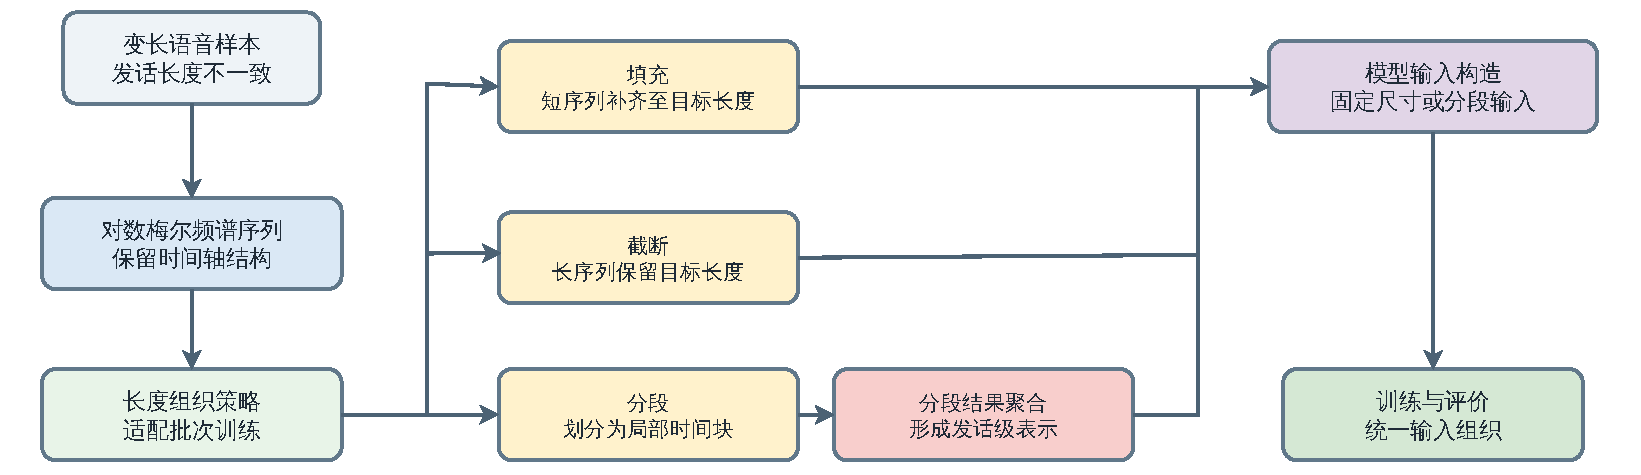
\includegraphics[width=\textwidth]{images/chapter2/chapter2_length_handling.drawio.pdf}
    \caption{变长语音特征的长度处理与输入组织方式}
    \label{fig:chapter2_length_handling}
\end{figure}

从语音情绪识别的视角来看，输入长度处理并非单纯的格式整理，还会影响情绪片段是否被充分保留。图\ref{fig:chapter2_length_handling}概括了三类常见处理方式及其输入组织差异。


% \subsection{数据增强与鲁棒性提升}



% \section{面临难点}

% 在语音情绪识别中，信号处理技术的必要性主要源于原始语音信号难以以规整、清晰的形式提供情绪信息\cite{lu2022domain,lin2023chunk}。语音情绪识别中的信号处理，可视为在噪声干扰环境下表征有效特征的重要环节\cite{gao2024adversarial,zhang2020transfer}。现有研究亦指出，语音情绪识别在数据集构成、特征提取、噪声环境、泛化能力等方面仍面临一定挑战\cite{su2023unsupervised,leem2024selective,peng2021efficient}。上述挑战主要体现在语音信号的非平稳性、发话长度可变性、外部环境干扰、情绪线索的多层性、用户与数据集的分布差异以及数据规模限制等方面。

% \begin{figure}[htbp]
%     \centering
%     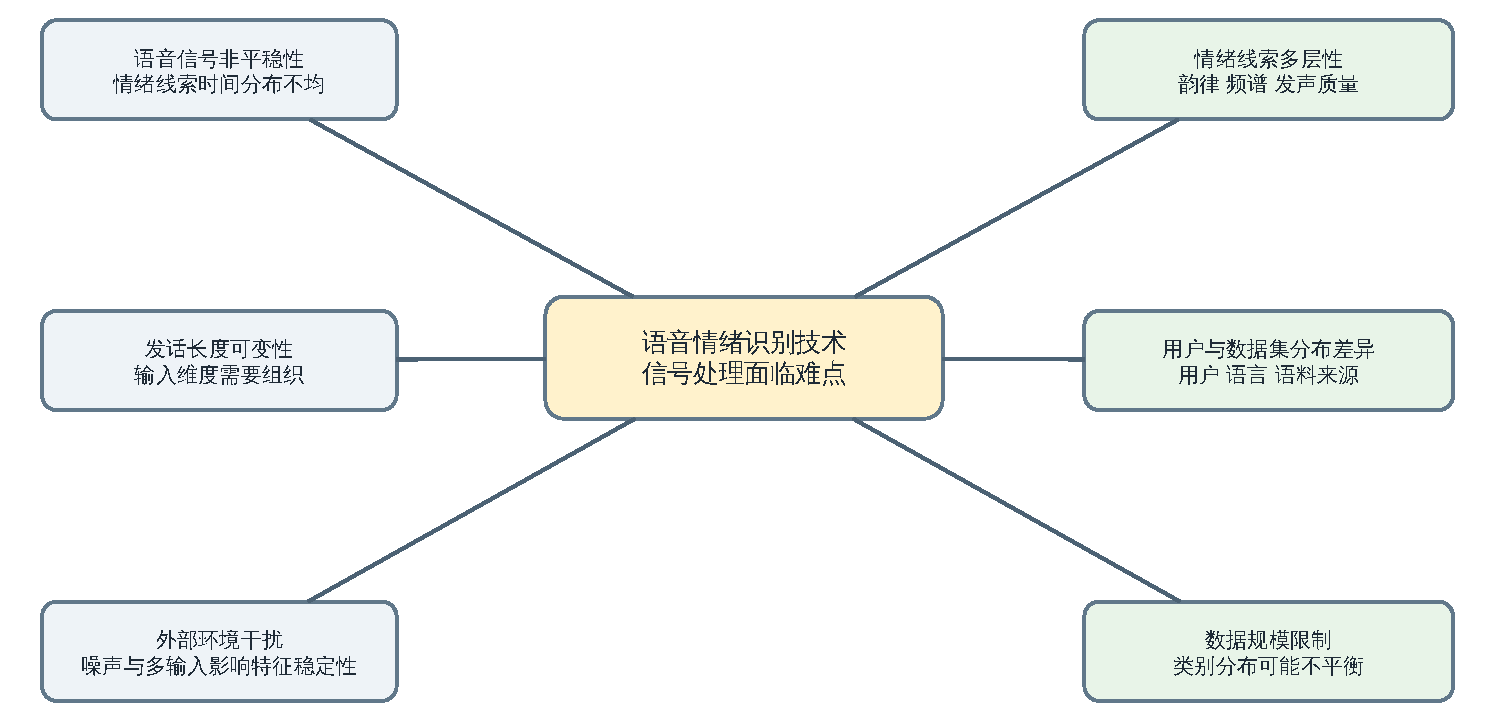
\includegraphics[width=0.92\textwidth]{images/chapter2/chapter2_ser_challenges_map.drawio.pdf}
%     \caption{语音情绪识别中信号处理面临的主要难点}
%     \label{fig:chapter2_ser_challenges_map}
% \end{figure}

% \subsection{语音信号的非平稳性与时间非均匀性}

% 语音信号的非平稳性与情绪线索的时间非均匀性，是语音情绪识别中较为基础的难点之一。语音在发话全程中并不保持统一的统计结构，音节边界、清浊音交替、语调升降、局部能量变化持续发生\cite{ma2023review,lin2023chunk}。情绪表达集中于发话中的特定区间，而非均匀分布于整个发话过程\cite{peng2021efficient}。例如，愤怒可能在特定单词的强调区间或重读音节中表现为较为明显的能量上升与基频变化；悲伤即便整体呈现低能量与慢语速，也可能在发话后半段表现出一定程度的语调下降或拖音。情绪信息在时间轴上的局部分布特性，使得将整个波形视为单一静态向量的处理方式难以充分保留信息。在语音情绪识别中，相较于“提取哪些特征”的问题，“采用何种时间单位进行分析才能避免遗漏情绪信息”是需要关注的问题。现有语音情绪识别综述亦指出，语音属于非平稳信号，情绪信息在不同时间区间呈现不同分布。基于短时分析的声学特征提取仍被视为关键环节。分帧、加窗、短时傅里叶变换、谱图、对数梅尔谱等短时时频分析技术，可视为应对上述问题的重要方法。

% \subsection{发话长度的可变性}

% 发话长度的可变性对语音情绪识别的实验设计与模型输入构成形成一定约束\cite{ma2023review,lin2023chunk}。语音情绪识别数据集中，不同发话的长度存在差异，即便在同一情绪类别内部，短时发话与较长发话也可能同时存在。这一差异影响后续特征提取，也会作用于模型学习结构。若直接使用长度不一的发话进行训练，批处理过程可能面临困难；在输入维度固定的模型中，未加处理的变长序列可能难以直接使用或效率较低。采用零填充统一长度时，若填充比例过高，输入中无意义零值区间的比重可能增大；采用截断时，发话后段蕴含的情绪线索可能被丢弃。将长时发话划分为多个分段或采用分段处理，有助于捕捉局部情绪信息，但需进一步设计分段结果的整合方式\cite{peng2021efficient}。近期面向分段级语音情绪识别的相关研究亦指出，将长时发话压缩为单一固定长度向量的处理方式存在一定局限。发话长度的可变性问题，可视为在情绪信息保留与模型输入一致性之间寻求平衡的重要方面。

% \subsection{外部环境因素的干扰}

% 噪声、多输入、信道差异等外部环境因素，在语音情绪识别中构成较为明显的干扰因素。实验室环境下录制的语音通常具有较为清晰的声学特征；实际应用场景中，噪声环境、人声或物体移动产生的杂音、室内多输入、麦克风质量差异、录音距离变化、压缩过程带来的信息损失等因素可能同时存在\cite{ma2023review,leem2024selective,lin2023chunk}。上述因素可能在语音信号中引入与情绪表达无直接关联的波动，改变能量分布与频谱结构，进而影响特征提取的稳定性\cite{zhang2020transfer}。情绪识别比语音识别更依赖细微声学差异，噪声水平相近时，情绪识别性能也可能受到更明显影响。例如，语调的微小上升、特定频带的能量增强、带有气息感的发声质感等，均可能成为判断情绪的重要线索，而这些线索可能受噪声与多输入干扰。近期面向噪声环境下的语音情绪识别研究及相关综述亦指出，噪声条件下情绪识别性能可能出现明显下降，实际应用中需结合去噪处理、鲁棒特征设计及数据增强等策略加以应对\cite{peng2021efficient}。语音情绪识别中的信号处理不应只以理想化、无干扰的输入为前提，还需要纳入实际环境中可能出现的声学失真。

% \subsection{情绪线索的多层性与特征表示的复杂性}

% 情绪线索的多层性与特征表示的复杂性，是语音情绪识别中较为突出的难点之一\cite{ma2023review,pappagari2023music,peng2021efficient}。情绪变化会表现为基频升高或能量增强等单一声学维度的波动，也会体现为多种声学维度的协同变化。某些情绪可能在语调与语速变化中体现得更为明显，另一些情绪则可能更多反映在频谱包络、共振峰结构、倒谱特性、嗓音质量、气息感、粗糙度等较为精细的声学特征之中。上述韵律、频谱、倒谱、嗓音质量等多类信息在情绪表达中相互叠加与交互，使得依赖单一特征表示可能难以充分区分不同情绪类别。例如，梅尔频率倒谱系数能够较好地概括频谱包络，但难以直接反映基频轮廓与时长模式的变化；基频、能量等韵律特征虽易于解释，却难以涵盖频谱差异或发声质感等维度。现有研究中反复探讨多特征组合、特征选择与特征融合等问题，反映了这一复杂性。语音情绪识别中的关键挑战不宜简化为寻找单一“较优”特征；更需要关注如何设计能够尽可能保留情绪多层结构的输入表示方式。上述问题为后续讨论对数梅尔谱、梅尔频率倒谱系数、韵律特征及特征集（如OpenSMILE）等技术提供了问题背景。

% \subsection{用户、语言及数据集的分布差异}

% 用户差异、语言差异及数据集间的分布差异，与情绪本身的差异相互交织，构成语音情绪识别中的复杂问题之一\cite{ma2023review,lin2023chunk,peng2021efficient}。即便表达同一情绪，不同用户的基频范围、语速、重音模式、能量水平、发音习惯等方面可能存在差异。语言背景不同时，语调结构、音节节奏、长短音体系、重音实现方式等也会随之变化。不同数据集在录音环境、用户构成、情绪标签体系、表演型或自然型语音的选取等方面存在差异。在某一数据集上表现良好的输入表示或特征组合，在另一数据集上未必能保持相同性能\cite{leem2024selective}。情绪变化与用户、语言、领域等因素引起的声学变化相互叠加，这两类变化在信号处理阶段较难完全分离。例如，直接使用基频或能量的绝对值，可能更多反映用户差异而非情绪差异。许多研究同时关注按发话单元归一化、按语料库归一化、用户独立性及跨语料库鲁棒性等问题。相关综述亦指出，在用户独立与跨语料库设定下，情绪识别性能可能出现较为明显的下降。语音情绪识别中的信号处理涉及特征提取的准确性，也需关注如何在一定程度上减少用户与领域带来的无关波动\cite{zhang2020transfer}。

% \subsection{情绪数据的规模限制与类别不平衡}

% 情绪数据的规模限制与类别不平衡问题，在信号处理阶段形成一定约束\cite{ma2023review,lin2023chunk,peng2021efficient}。相较于通用语音识别数据，带有情绪标签的语音数据收集成本较高，标注一致性也较难保障。实际研究中使用的数据集在用户数量与发话数量上往往较为有限，部分情绪类别的样本数量可能较少，类别分布也可能存在一定程度的不平衡。在此类条件下，若输入特征维度过高，或引入与数据规模不相适应的复杂处理流程，可能增加过拟合风险；反之，若特征过度简化，则可能丢失与情绪相关的重要信息。近期研究亦指出，样本不足、特征维度过高、无关特征过多等因素可能影响语音情绪识别能力，为此常通过特征选择、数据增强及鲁棒表示设计等方式加以应对\cite{liu2023dualrobustness}。信号处理阶段不应该仅追求理论上的信息丰富性，而应综合考虑实际数据条件与学习稳定性，选择适当的处理复杂度\cite{fan2022isnet,zhang2020transfer}。


\section{现有技术}

语音情绪识别领域的信号处理技术，可根据输入语音转换为何种特征表示，划分为若干改进方向\cite{ma2023review,lin2023chunk,peng2021efficient}。第一种改进方向采用人工设计的固定变换特征。该类方法从语音信号中提取梅尔频率倒谱系数、对数梅尔谱、谱图、基频、能量、共振峰等特征。第二种改进方向利用大规模无标注语音数据中学习的特征表示。该类方法使用 Wav2Vec2、HuBERT、WavLM 等自监督学习模型，从原始语音中提取高维特征向量\cite{thanh2024robust,sampath2025efficient}。第三种改进方向聚焦于信号的鲁棒性。该类方法采用噪声添加、多输入添加、数据增强、去噪处理、特征增强等技术\cite{leem2024selective}。

第一种改进方向采用人工设计的固定变换特征，主要包括谱图、对数梅尔谱图、梅尔频率倒谱系数等时频域特征，以及基频、能量、共振峰等韵律与发声质量特征\cite{ma2023review,peng2021efficient}。代表性特征集包括基于OpenSMILE提取的eGeMAPS、ComParE等，常用于基准对比。该类特征可解释性较强，但依赖先验设计，难以通过单一固定特征集完整捕捉情绪的复杂表达\cite{pappagari2023music}。

第二种改进方向利用大规模无标注语音数据训练的自监督学习模型提取高维特征表示，代表性模型包括Wav2Vec2、HuBERT和WavLM等\cite{baevski2020wav2vec2,hsu2021hubert,chen2022wavlm}。自监督学习特征在语音情绪识别的下游研究中表现出较强潜力\cite{pepino2021wav2vec,fang2023downstreamssl,thanh2024robust}，但模型规模较大、计算资源消耗较高，预训练目标与情绪识别需求之间可能存在差异\cite{sampath2025efficient,feng2023peftser}。

第三种改进方向关注信号的鲁棒性，采用噪声添加、速度扰动等数据增强技术、前处理阶段的去噪算法或特征提取阶段的鲁棒特征设计，以提高模型在噪声环境和多输入等实际条件下的稳定性\cite{leem2024selective,thanh2024robust,tzeng2025noiserobust}。


\section{本文采用的信号处理流程}

结合前文对数据集、信号处理技术和任务难点的分析，本文实验采用以对数梅尔频谱为中心的信号处理流程。该流程不直接使用原始波形作为分类器输入，也不引入大规模自监督语音模型提取高维表示。实验先将语音整理为具有明确时频含义的二维表示，再根据不同模型的输入接口完成尺寸整理或分块组织。这样的安排有助于在计算成本、特征可解释性和模型比较一致性之间取得相对平衡\cite{ma2023review,lin2023chunk,peng2021efficient}。

\begin{figure}[htbp]
    \centering
    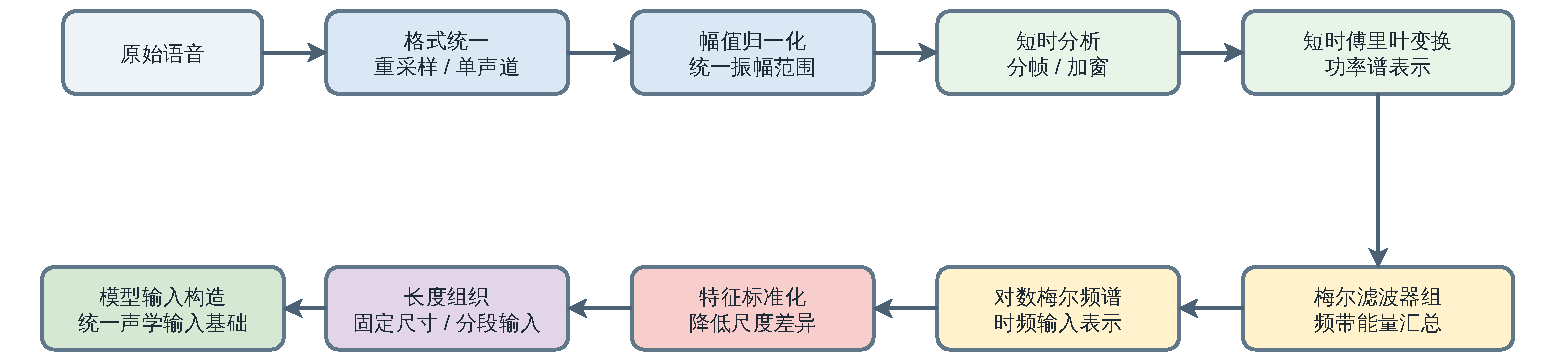
\includegraphics[width=\textwidth]{images/chapter2/chapter2_signal_processing_pipeline.drawio.pdf}
    \caption{本文采用的信号处理流程}
    \label{fig:chapter2_signal_processing_pipeline}
\end{figure}

图\ref{fig:chapter2_signal_processing_pipeline}汇总了本文从原始语音到模型输入的信号处理流程。该流程依次包含格式统一、幅值归一化、短时分析、功率谱表示、梅尔滤波、对数梅尔频谱、特征标准化和长度组织，后续四个小段按照该顺序展开说明。

\textbf{(1) 输入格式统一与幅值归一化。}

本文首先对原始语音进行格式统一处理。RAVDESS语音样本原始采样率较高，实验流程中将语音统一重采样到16kHz，并保持单声道输入形式。采样率统一后，不同语音样本在后续短时分析中具有一致的时间刻度。幅值归一化用于降低录音音量差异对特征提取的影响，使后续频谱能量分布更多反映发话本身的声学变化，而不是文件级音量尺度差异\cite{ma2023review,lin2023chunk}。

\textbf{(2) 对数梅尔频谱提取。}

完成基础预处理后，本文采用短时傅里叶变换和梅尔滤波器组提取对数梅尔频谱。实验流程保留固定的快速傅里叶变换长度、帧移与频率范围设置，使不同样本在后续模型比较中具有一致的时频分析口径。对数梅尔频谱既保留语音在时间轴上的局部变化，又将频率轴整理为接近听觉感知的频带表示，适合作为卷积神经网络、Transformer和CNN-Conformer模型的共同输入基础\cite{ma2023review,peng2021efficient}。

\textbf{(3) 特征标准化与输入长度组织。}

对数梅尔频谱提取后，本文对特征进行标准化处理，以降低不同样本之间整体能量尺度差异带来的影响。由于语音样本长度不完全一致，输入长度处理根据模型结构有所区分。卷积神经网络基线模型采用固定尺寸谱图输入，便于与二维卷积分类器相适配；CNN-Conformer代表配置则采用分块组织方式，将发话按固定帧数整理为局部时间块，再在推理阶段聚合得到发话级结果。上述处理方式使模型能够在控制显存开销的同时保留较多局部时间信息\cite{lin2023chunk,peng2021efficient}。

\textbf{(4) 训练阶段的有限增强处理。}

在训练阶段，本文保留较为克制的数据增强策略。对CNN-Conformer代表配置，实验采用频谱级混合增强，在训练样本及其标签之间进行线性插值，降低模型对少量训练样本或特定用户声学模式的依赖。该处理属于训练阶段的正则化技术，不改变推理阶段的输入流程。噪声条件实验在模型选择完成后作为补充评价进行，噪声只在评价波形阶段加入，用于观察已选代表模型在受扰输入下的变化情况\cite{kang2023labelmixup,leem2024selective,zhou2020using}。

通过上述处理，本文形成了从原始语音到模型输入的统一流程：语音格式统一、幅值归一化、对数梅尔频谱提取、特征标准化、长度组织与模型输入构造。该流程为第四章中的三类模型比较提供相同的声学输入基础，也为后续噪声条件和跨语料库评价保留了可复现的前处理口径。





\section{本章小结}

本章围绕语音情绪识别中的数据集选择与信号处理技术展开说明。首先，本章比较了常见语音情绪数据集的来源、规模、标签体系和适用条件，并结合用户数量、类别覆盖和实验可复现性，确定RAVDESS语音情绪数据集作为本文主要实验对象。数据集选择为后续用户无关划分、模型比较和类别层面分析提供了实验基础。

随后，本章从信号预处理、时频变换、感知特征提取、特征后处理与序列长度处理等方面整理了语音情绪识别中常用的信号处理技术。语音信号具有非平稳性和长度可变性，情绪线索又分布在能量、频谱、韵律和发声质量等多个层面。短时傅里叶变换、对数梅尔频谱、梅尔频率倒谱系数、归一化和分段处理等技术，可将原始波形转化为较适合模型学习的输入表示。

在此基础上，本章归纳了语音情绪识别面临的主要难点，包括外部环境干扰、用户与数据集分布差异、数据规模限制和类别不平衡等问题。现有技术通常从人工设计声学特征、自监督语音表示和鲁棒性增强三个方向展开。结合本文的实验条件，后续章节采用以对数梅尔频谱为中心的信号处理流程，并在相同输入基础上比较卷积神经网络基线模型、纯Transformer模型和CNN-Conformer模型的表现。
